\documentclass[a4paper,12pt]{article}
\usepackage{xcolor}
\usepackage{amsmath}
\usepackage{hyperref}
\usepackage{graphicx}
\usepackage{float}
\usepackage{subcaption}
\usepackage{listings}
\usepackage{circuitikz}
\usepackage{titling}

\pretitle{\begin{center}\Huge\bfseries\color{blue}}
\posttitle{\par\end{center}\vskip 0.5em}
\preauthor{\begin{center}\Large\color{red}}
\postauthor{\par\end{center}\vskip 0.5em}
\predate{\begin{center}\large\color{green}}
\postdate{\par\end{center}\vskip 1em}



\begin{document}


\begin{titlepage}
    \centering
    \vspace*{1cm}
    \Huge \textbf{Lab Report 5: Op-Amp Applications}
    \vspace{1.5cm}
    
    \LARGE \textbf{Submitted By:}\\
    \Large Krishna Patil (EE24BTECH11036)\\
    Deepak Kumar Ahirwar (EE24BTECH11014)
    
    \vfill
    
    \Large \textbf{Department of Electrical Engineering}\\
    \Large \textbf{IIT Hyderabad}\\
    \Large \today
    
    \vspace*{2cm}
\end{titlepage}

\section*{Objective}
\textcolor{blue}{To study the applications of operational amplifiers (Op-Amps) by implementing:}
\begin{itemize}
    \item \textcolor{red}{Custom weighted summing and difference amplifier}
    \item \textcolor{red}{Op-Amp integrator}
    \item \textcolor{red}{Precision rectifier (Super Diode)}
\end{itemize}

\section*{Apparatus}
\begin{itemize}
    \item \textcolor{blue}{Operational Amplifiers (LM358, LM741, TL081)}
    \item \textcolor{blue}{Resistors (selected for proper weighting and circuit operation)}
    \item \textcolor{blue}{Capacitors (for integration circuit)}
    \item \textcolor{blue}{Diodes (e.g., 1N4148 for rectification)}
    \item \textcolor{blue}{DC power supply}
    \item \textcolor{blue}{Function generator}
    \item \textcolor{blue}{Oscilloscope}
\end{itemize}

\section*{Theory}
\subsection*{\textcolor{blue}{1. Custom Weighted Summing and Difference Amplifier}}
A summing amplifier combines multiple inputs with specified gains. Using an inverting summing amplifier configuration:
\begin{equation}
V_{out} = -\left(\frac{R_f}{R_1}V_1 + \frac{R_f}{R_2}V_2 + \frac{R_f}{R_3}V_3\right)
\end{equation}
For specific resistor values, the desired expressions can be achieved:
\begin{equation}
V_{out} = 2V_1 + V_2 - V_3
\end{equation}
\begin{equation}
V_{out} = 2V_1 - V_3
\end{equation}

\begin{figure}[H]
    \centering
    
\begin{circuitikz}
\tikzstyle{every node}=[font=\large]

\draw (12.75,11.25) node[op amp,scale=1, yscale=-1 ] (opamp2) {};
\draw (opamp2.+) to[short] (11.25,11.75);
\draw  (opamp2.-) to[short] (11.25,10.75);
\draw (13.95,11.25) to[short](14.25,11.25);
\draw (13.25,9.25) to[short] (13.75,9.25);
\node at (15.75,11.25) [circ] {};
\draw (15.75,11.25) to[short, -o] (17.75,11.25) ;
\node [font=\large] at (18.75,11.5) {$V_{out}$};
\draw (11.25,10.75) to[short] (11.25,9.25);
\draw (11.25,9.25) to[short] (13.5,9.25);
\draw (13.75,11.25) to[D] (15.75,11.25);
\draw (13.75,9.25) to[short] (15.75,9.25);
\draw (15.75,9.25) to[short] (15.75,11.25);
\draw (17,11.25) to[R] (17,9.25);
\draw (17,9.25) to (17,8.75) node[ground]{};
\node [font=\large] at (11.25,12.25) {$V_{in}$};
\node [font=\large] at (17.5,10.25) {$R_l$};
\end{circuitikz}

    \caption{Summing and Difference Amplifier Circuit}
\end{figure}

\subsection*{\textcolor{blue}{2. Op-Amp Integrator}}
An Op-Amp integrator mathematically integrates the input signal:
\begin{equation}
V_{out} = -\frac{1}{RC} \int V_{in} dt
\end{equation}
It converts a square wave input into a triangular wave output and is useful in signal processing applications.

\begin{figure}[H]
    \centering
    
\begin{circuitikz}
\tikzstyle{every node}=[font=\large]

\draw (12.75,11.25) node[op amp,scale=1, yscale=-1 ] (opamp2) {};
\draw (opamp2.+) to[short] (11.25,11.75);
\draw  (opamp2.-) to[short] (11.25,10.75);
\draw (13.95,11.25) to[short](14.25,11.25);
\draw (13.25,9.25) to[short] (13.75,9.25);
\node at (15.75,11.25) [circ] {};
\draw (15.75,11.25) to[short, -o] (17.75,11.25) ;
\node [font=\large] at (18.75,11.5) {$V_{out}$};
\draw (11.25,10.75) to[short] (11.25,9.25);
\draw (11.25,9.25) to[short] (13.5,9.25);
\draw (13.75,11.25) to[D] (15.75,11.25);
\draw (13.75,9.25) to[short] (15.75,9.25);
\draw (15.75,9.25) to[short] (15.75,11.25);
\draw (17,11.25) to[R] (17,9.25);
\draw (17,9.25) to (17,8.75) node[ground]{};
\node [font=\large] at (11.25,12.25) {$V_{in}$};
\node [font=\large] at (17.5,10.25) {$R_l$};
\end{circuitikz}

    \caption{Op-Amp Integrator Circuit}
\end{figure}

\subsection*{\textcolor{blue}{3. Precision Rectifier (Super Diode)}}
A precision rectifier eliminates the 0.7V drop of standard diodes by using an Op-Amp:
\begin{equation}
V_{out} = \begin{cases} 0, & V_{in} < 0 \\ V_{in}, & V_{in} > 0 \end{cases}
\end{equation}
For a full-wave rectifier, an additional summing stage is used to combine positive and inverted negative portions.

\begin{figure}[H]
    \centering
    
\begin{circuitikz}
\tikzstyle{every node}=[font=\large]

\draw (12.75,11.25) node[op amp,scale=1, yscale=-1 ] (opamp2) {};
\draw (opamp2.+) to[short] (11.25,11.75);
\draw  (opamp2.-) to[short] (11.25,10.75);
\draw (13.95,11.25) to[short](14.25,11.25);
\draw (13.25,9.25) to[short] (13.75,9.25);
\node at (15.75,11.25) [circ] {};
\draw (15.75,11.25) to[short, -o] (17.75,11.25) ;
\node [font=\large] at (18.75,11.5) {$V_{out}$};
\draw (11.25,10.75) to[short] (11.25,9.25);
\draw (11.25,9.25) to[short] (13.5,9.25);
\draw (13.75,11.25) to[D] (15.75,11.25);
\draw (13.75,9.25) to[short] (15.75,9.25);
\draw (15.75,9.25) to[short] (15.75,11.25);
\draw (17,11.25) to[R] (17,9.25);
\draw (17,9.25) to (17,8.75) node[ground]{};
\node [font=\large] at (11.25,12.25) {$V_{in}$};
\node [font=\large] at (17.5,10.25) {$R_l$};
\end{circuitikz}

    \caption{Precision Rectifier Circuit}
\end{figure}

\section*{Procedure}
\begin{enumerate}
    \item Assemble each circuit as per the given schematics.
    \item Apply appropriate input signals using a function generator.
    \item Measure output using an oscilloscope.
    \item Compare theoretical and experimental results.
    \item Record observations and plot graphs.
\end{enumerate}

\section*{Observations}
\subsection*{Summing and Difference Amplifier}
$R_1=R_2=2k\Omega$, $R_3=1k\Omega$
\begin{figure}[H]
    \centering
    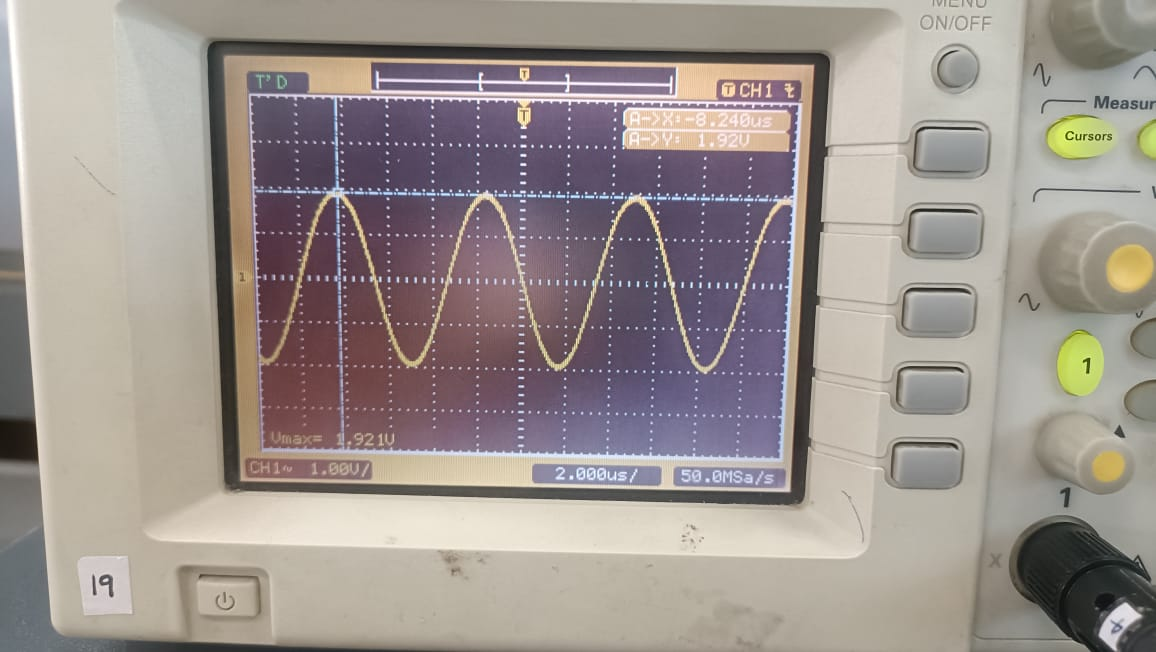
\includegraphics[width=0.7\textwidth]{figs/5.1/1.jpeg}
        \caption{$V_1=V_2=sin(2\pi ft)$ $f=150kHz$}
\end{figure}
\begin{figure}[H]
    \centering
    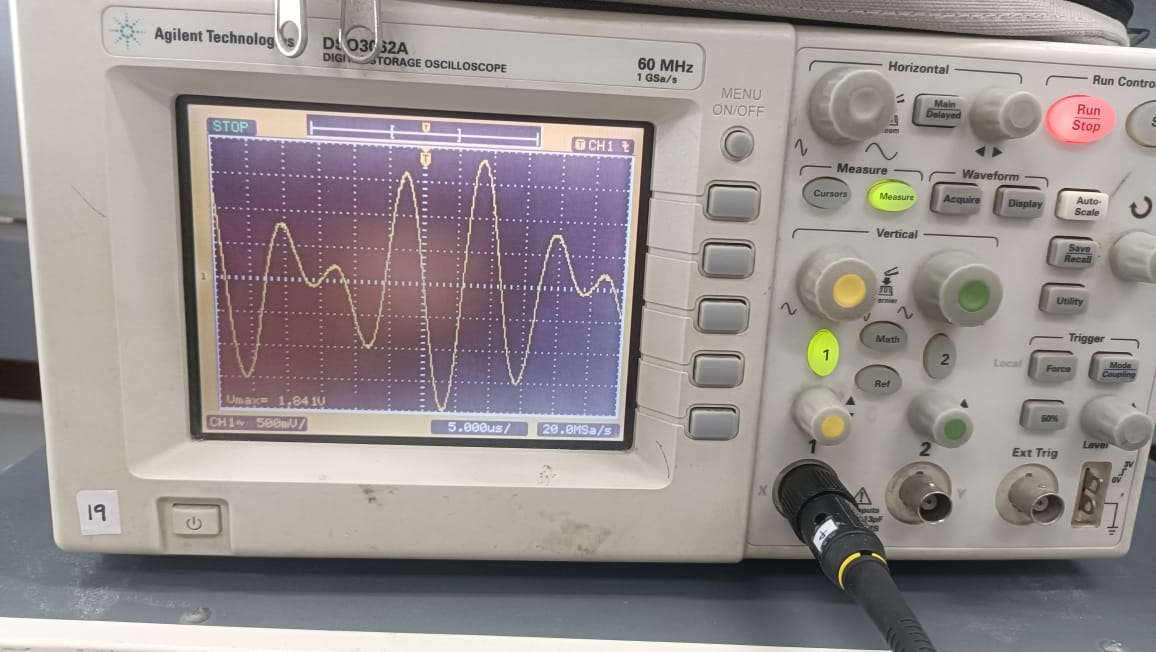
\includegraphics[width=0.7\textwidth]{figs/5.1/2.jpeg}
        \caption{$V_1=sin(2\pi f_1t), V_2=sin(2\pi f_2t), f_1=75kHz, f_2=100kHz$}
\end{figure}
\begin{figure}[H]
    \centering
    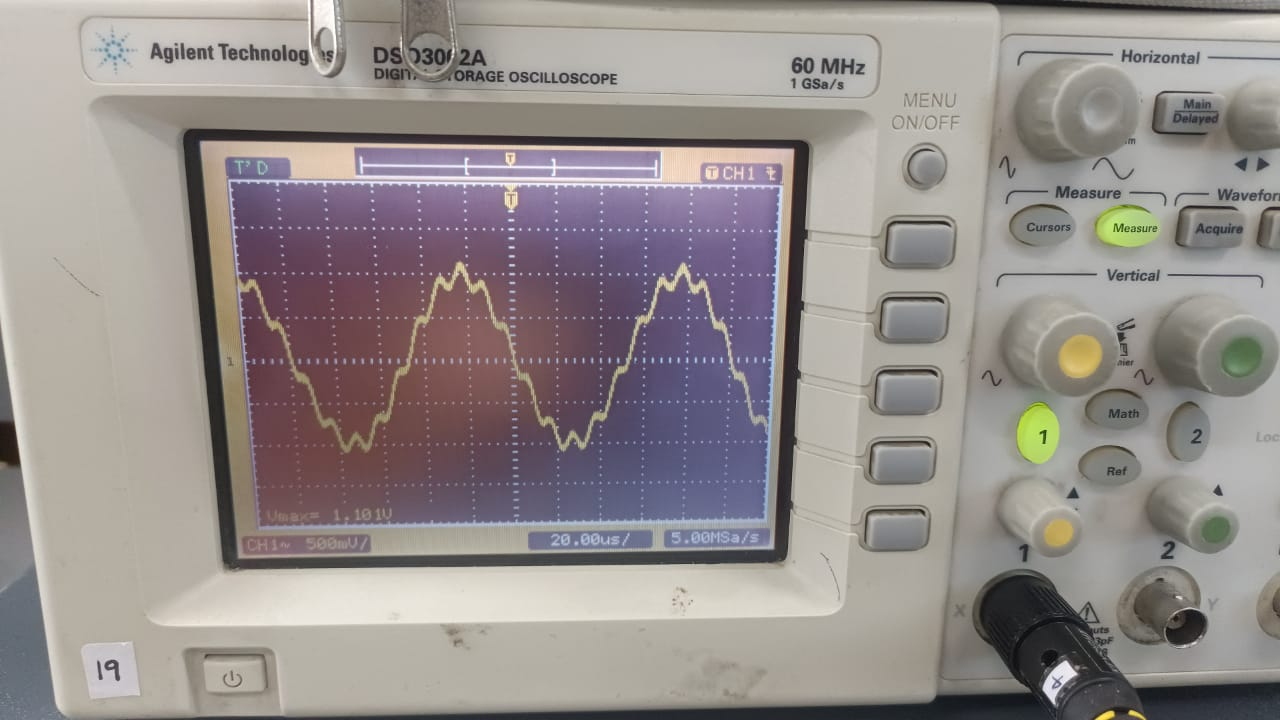
\includegraphics[width=0.7\textwidth]{figs/5.1/3.jpeg}
\end{figure}


\subsection*{Op-Amp Integrator}
\begin{figure}[H]
    \centering
    \begin{subfigure}{0.5\textwidth}
        \centering
        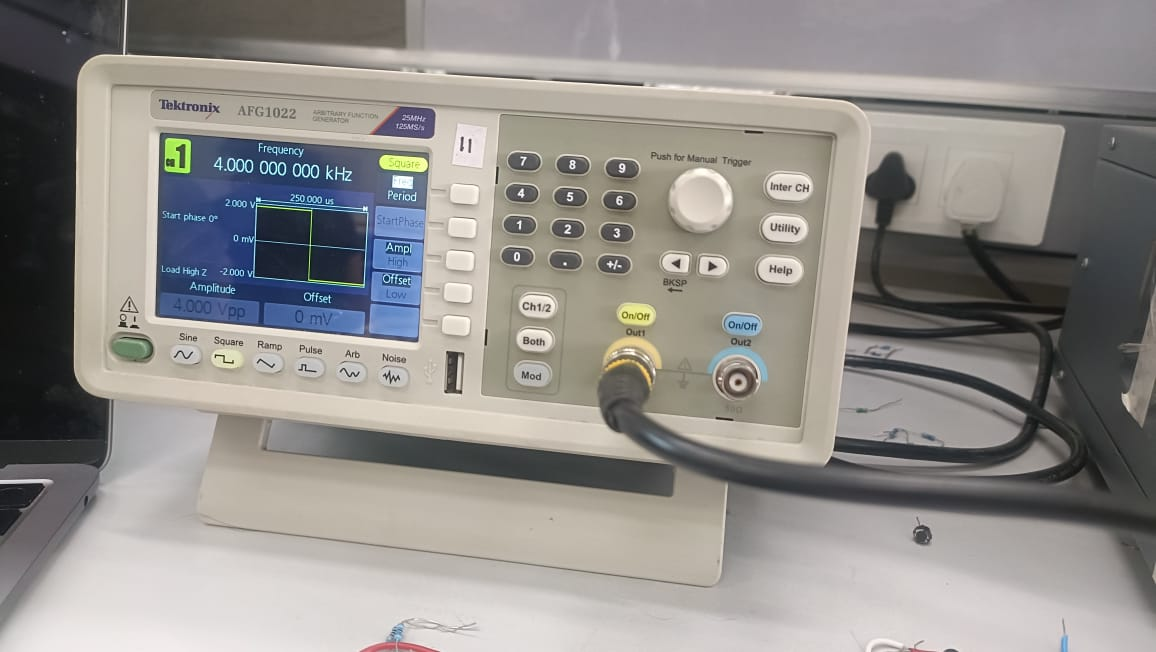
\includegraphics[height=5cm]{figs/5.2/para.jpeg}
    \end{subfigure}%
    \begin{subfigure}{0.5\textwidth}
        \centering
        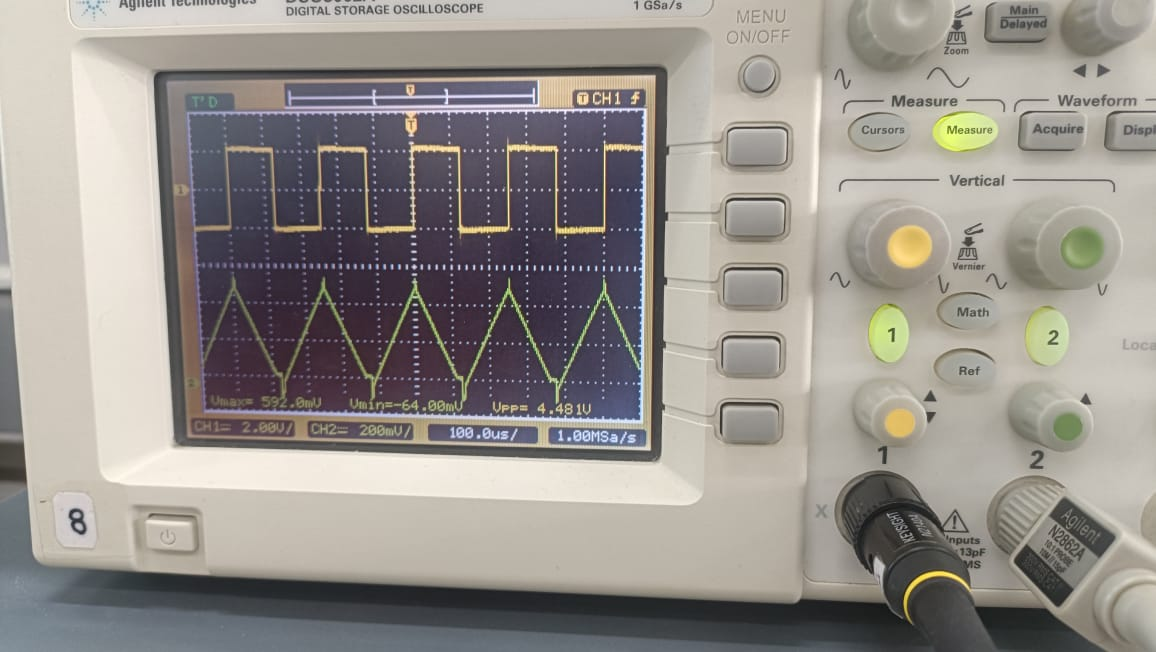
\includegraphics[height=5cm]{figs/5.2/plot.jpeg}
    \end{subfigure}
\end{figure}

\subsection*{Precision Rectifier}
\begin{figure}[H]
    \centering
    \begin{subfigure}{0.5\textwidth}
        \centering
        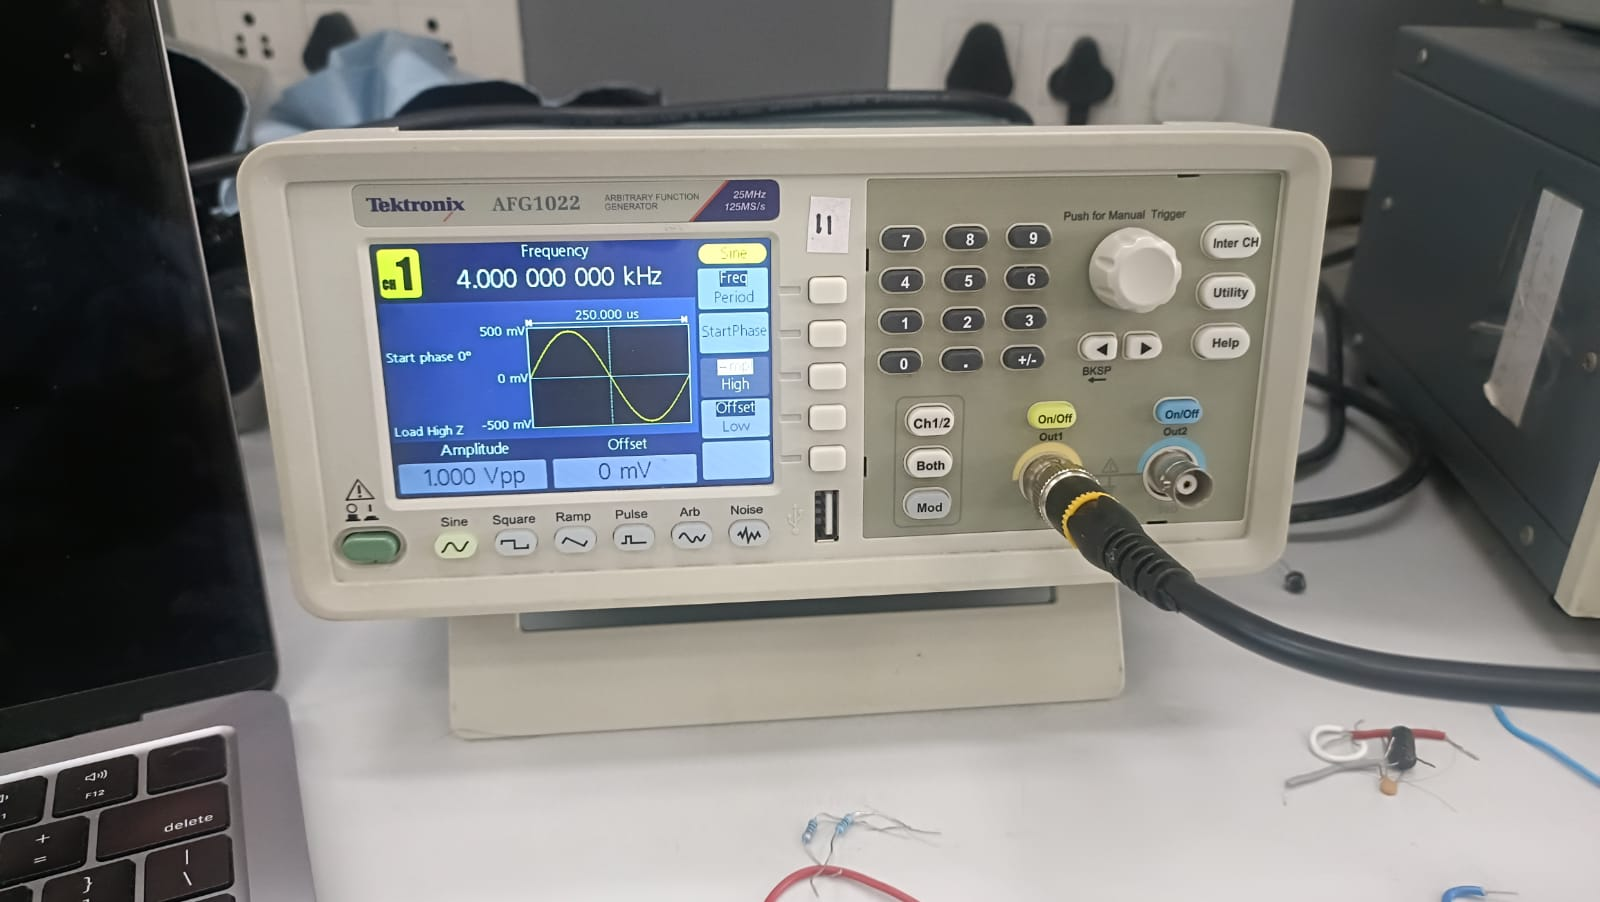
\includegraphics[height=5cm]{figs/5.3/para.jpeg}
    \end{subfigure}%
    \begin{subfigure}{0.5\textwidth}
        \centering
        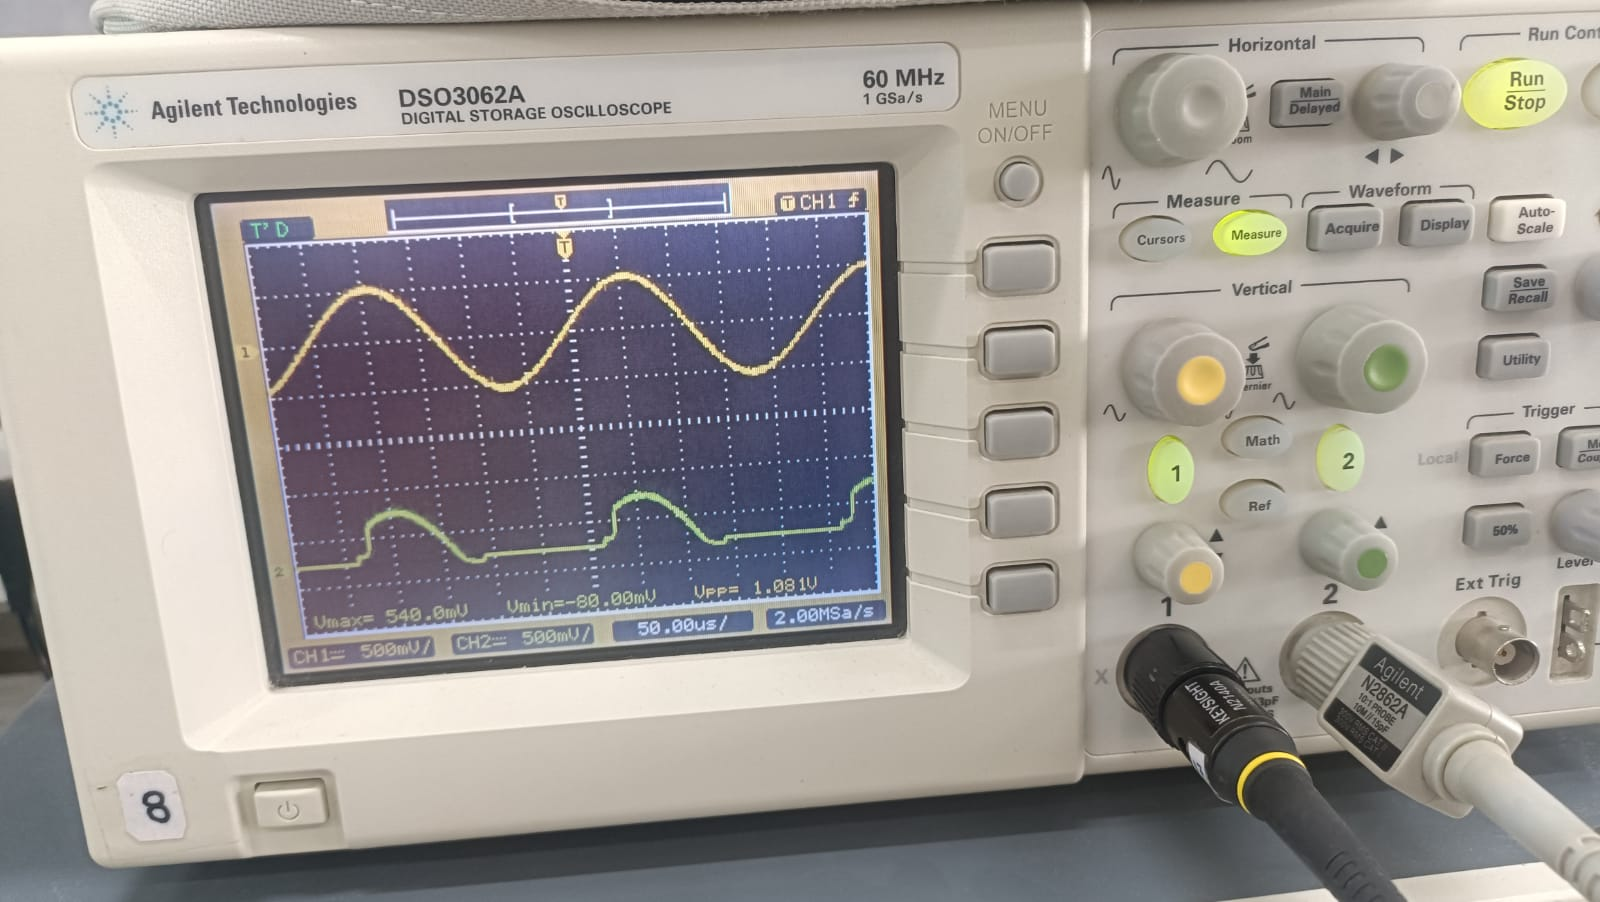
\includegraphics[height=5cm]{figs/5.3/plot.jpeg}
    \end{subfigure}
\end{figure}


\end{document}

